\documentclass[letterpaper,12pt]{article}
\usepackage{listings} %For code in appendix
\usepackage{color}
\usepackage{appendix}
\usepackage{tabularx} % extra features for tabular environment
\usepackage{amsmath}  % improve math presentation
\usepackage{graphicx} % takes care of graphic including machinery
\usepackage[margin=1in,letterpaper]{geometry} % decreases margins
\usepackage{cite} % takes care of citations
\usepackage[final]{hyperref} % adds hyper links inside the generated pdf file
\usepackage{float}
%\usepackage{pythonhighlight}

\hypersetup{
	colorlinks=true,       % false: boxed links; true: colored links
	linkcolor=blue,        % color of internal links
	citecolor=blue,        % color of links to bibliography
	filecolor=magenta,     % color of file links
	urlcolor=blue         
}
\usepackage{blindtext}

\lstset
{ %Formatting for code in appendix
    language=Python,
    basicstyle=\footnotesize,
    numbers=left,
    stepnumber=1,
    showstringspaces=false,
    tabsize=1,
    breaklines=true,
    breakatwhitespace=false,
}
%++++++++++++++++++++++++++++++++++++++++


\begin{document}
\title{DAT510-1 20H Network security and vulnerability. Assignment 2. Implement Secure Communications}
\author{Asahi Cantu Moreno (student id: 253964)}
\date{\today}
\maketitle

\begin{abstract}
Having knowledge on the way symmetric algorithms are implemented and work, this report focuses now on the theoretical explanation and results for the implementation of a secure framework for message transmission by applying several encryption and secure mechanisms which although simple, clearly describe the way real application work. The work and developed tasks are described in 2 parts:
\begin{enumerate}
    \item \textbf{Part I. Secure Communication Algorithm implementation.}
    Implementing algorithms for:
    \begin{itemize}
        \item Secure Key Exchange algorithm. Diffie-Hellman Key exchange method.
        \item CSPRNG\footnote{CSPRNG stands for Cryptography secure pseudo random number generator }  Implementing BBS\footnote{BBS is the Blum Blum Shub CSPRNG} generator
    \end{itemize}
    
    \item \textbf{Part II. Server and client implementation for secure communication.} A simple but real life implementation for secure messaging simulating the key exchange mechanisms and sending encrypted messages through the network.
\end{enumerate}
For each part a detailed explanation and emulation is provided, the workflow for key exchange and message encryption as well as demonstration of the application.
The developed code and implementations for each part of the assignment can be found together in the contents of this document repository.
\end{abstract}
\newpage

\section{Design and implementation}
\subsection{Part I. Secure Communication Algorithm implementation.}
\subsubsection{Diffie-Hellman Key Exchange algorithm}
The first published public-key algorithm appeared in the seminal paper by Diffie
and Hellman that defined public-key cryptography [DIFF76b] and is generally referred to as Diffie–Hellman key exchange. A number of commercial products employ this key exchange technique\cite{WS2017-SDES}. This algorithm allows two users to exchange their public key and send encrypted information without the need of sharing nor sending he private key.

The core of such algorithm relies on its ability to find the primitive root\footnote{A primitive root mod n is an integer g such that every integer relatively prime to n is congruent to a power of g mod n. The integer g is a primitive root (mod n) if for every number a relatively prime to n there is an integer z such that  $a \equiv g^z \mod n$} of a given prime number. Its effectiveness then relies on the difficulty to compute the discrete logarithm. Figure \ref{fig:DH} illustrates with more detail the key exchange method..

\begin{figure}[H]
    \centering
    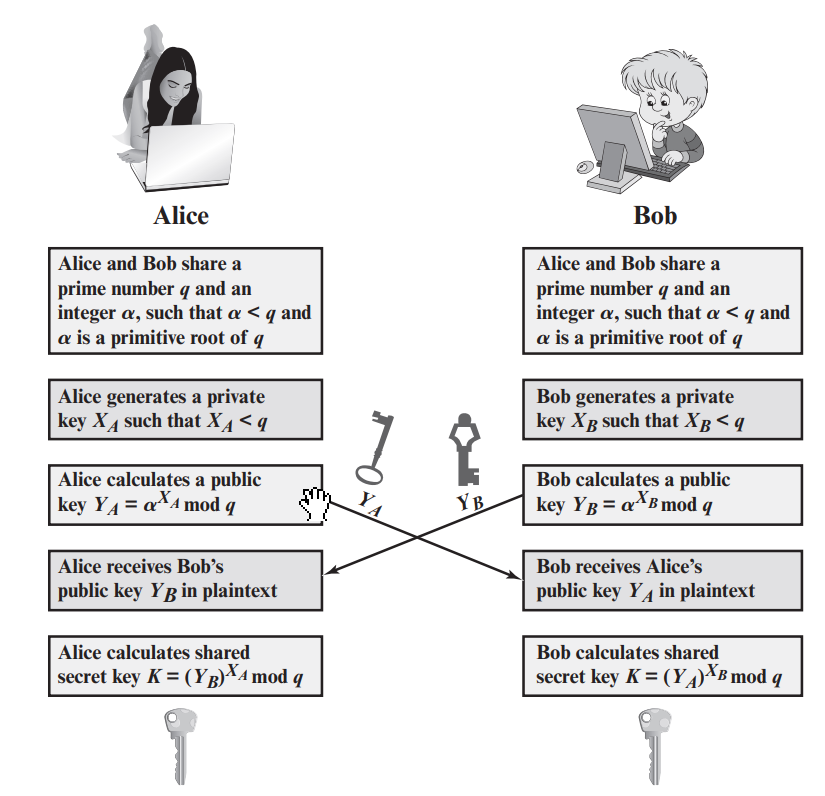
\includegraphics[width=0.7\textwidth]{assets/diffie_hellman.png}
    \caption{Diffie-Hellman algorithm explained.\cite{WS2017-SDES}}
    \label{fig:DH}
\end{figure}

Once the public keys are shared and shared keys submitted to each one of the users, the message can be generated, encrypted and send one to another. The decryption mechanism will then work without having to share the private key. This method was strengthened and enriched by randomly generating a private key by using a CSPRNG-BBS implementation. Once the message is sent, a new seed is created and passed to the BBS generator so a new random prime number can be emitted and later on used as a new private key. Once this is done the shared keys have to be generated and sent to the corresponding users.

The Blum Blum Shub random number generator was chosen for its simplicity on its implementation and reliability towards the generation of random numbers.

\subsubsection{Code implementation}
To perform all the requirements for this part I the algorithm and methodologies were developed using python language and some additional packages which can be found under the source code of this section.
\subsubsubsection{Python files created:}
\begin{enumerate}
    \item DH.py - Contains the implementation of Diffie-Hellman key exchange methodology
    \item BBS.py - Contains the implementation of Blum Blum Shug CSPRNG to regenerate the private keys
    
Finally a simulation for key sharing and message exchange through encryption was written. Log information can be shown in figure \ref{fig:DH_LOG}.
\end{enumerate}
\subsubsubsection{Key Exchange code simulation}
\hline
\begin{lstlisting}
import importlib
from DH import DH
from BBS import BBS
import sympy
import random
from Cryptodome.Cipher import AES
key_1 = sympy.randprime(2**17,2**18)
key_2 = DH.primRoots(key_1)[0]
dh_a = DH(key_2,key_1)
dh_b = DH(key_2,key_1)
messages = ['Hello World','This is a secret message','come here']
for message in messages:
    dh_a.create_shared_key()
    dh_b.create_shared_key()
    dh_a.create_full_key(dh_b.shared_key)
    dh_b.create_full_key(dh_a.shared_key)
    enc = dh_a.encrypt(message)
    dec = dh_b.decrypt(enc)
    dh_a.next_key()
    dh_b.next_key()
\end{lstlisting}
\hline


\subsection{Part II. Implementation of Secure Chat messenger.}
By confirming the developed algorithm works it was now required to implement a simple chat application that operates with the key exchange and encryption mechanisms previously developed.
For this implementation the same methodology as in Part I applies, with the creation of a server and client applications.
\subsubsection{Code Implementation}
\subsubsubsection{Python files created}
\begin{enumerate}
    \item Server.py: Is the server application. Runs in python with flask package and uses socketio communication protocol. The server just allows client-to-client communication by redirecting to the right session the messages and key exchanges. During the log session in the server it is possible to visualize that in any time the messaging information always is received encrypted and the only visible data are the public and shared keys.
    \item Client.py. Is the client application: Runs in python with Graphical User Interface and a socketio communication. It was thought in the beginning to develop the client side on a web page, but the main difficulty on doing that relied on the technology from which the algorithms were implemented, in this case, python. Having chosen web development would have meant to re-code in a different language such as JavaScript or make the application more complex otherwise. The graphical code was created using wxpython and employing the same encryption as in Part I.
\end{enumerate}

In figure \ref{fig:CRP_CHAT} a simulation of the program shows the results of the messaging exchange system.

\begin{figure}[H]
    \centering
    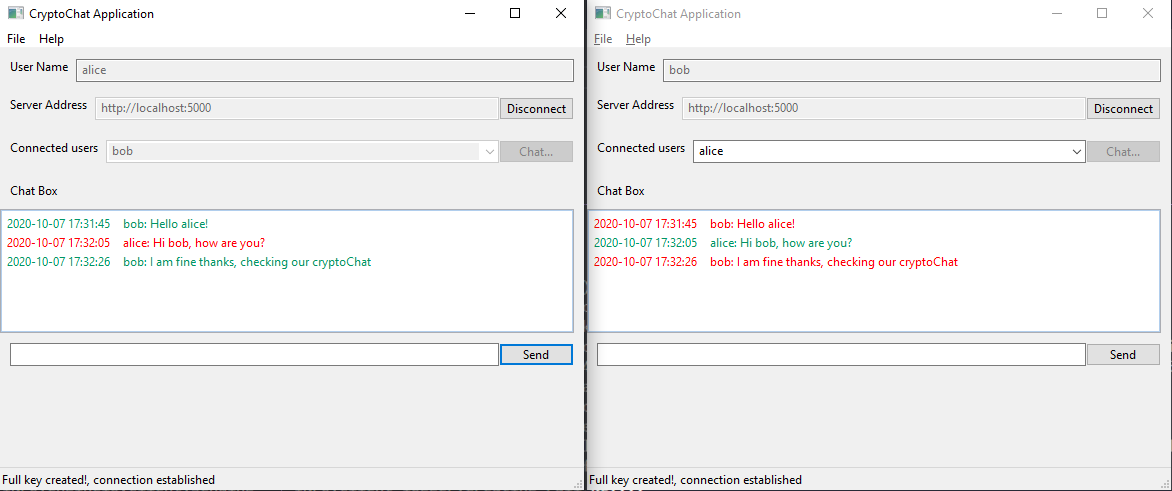
\includegraphics[width=0.9\textwidth]{assets/cryptochat.png}
    \caption{The log generated through running the emulated key exchange code.}
    \label{fig:CRP_CHAT}
\end{figure}

\section{Test Results}

\subsection{Part I Log generation}

\begin{figure}[H]
    \centering
    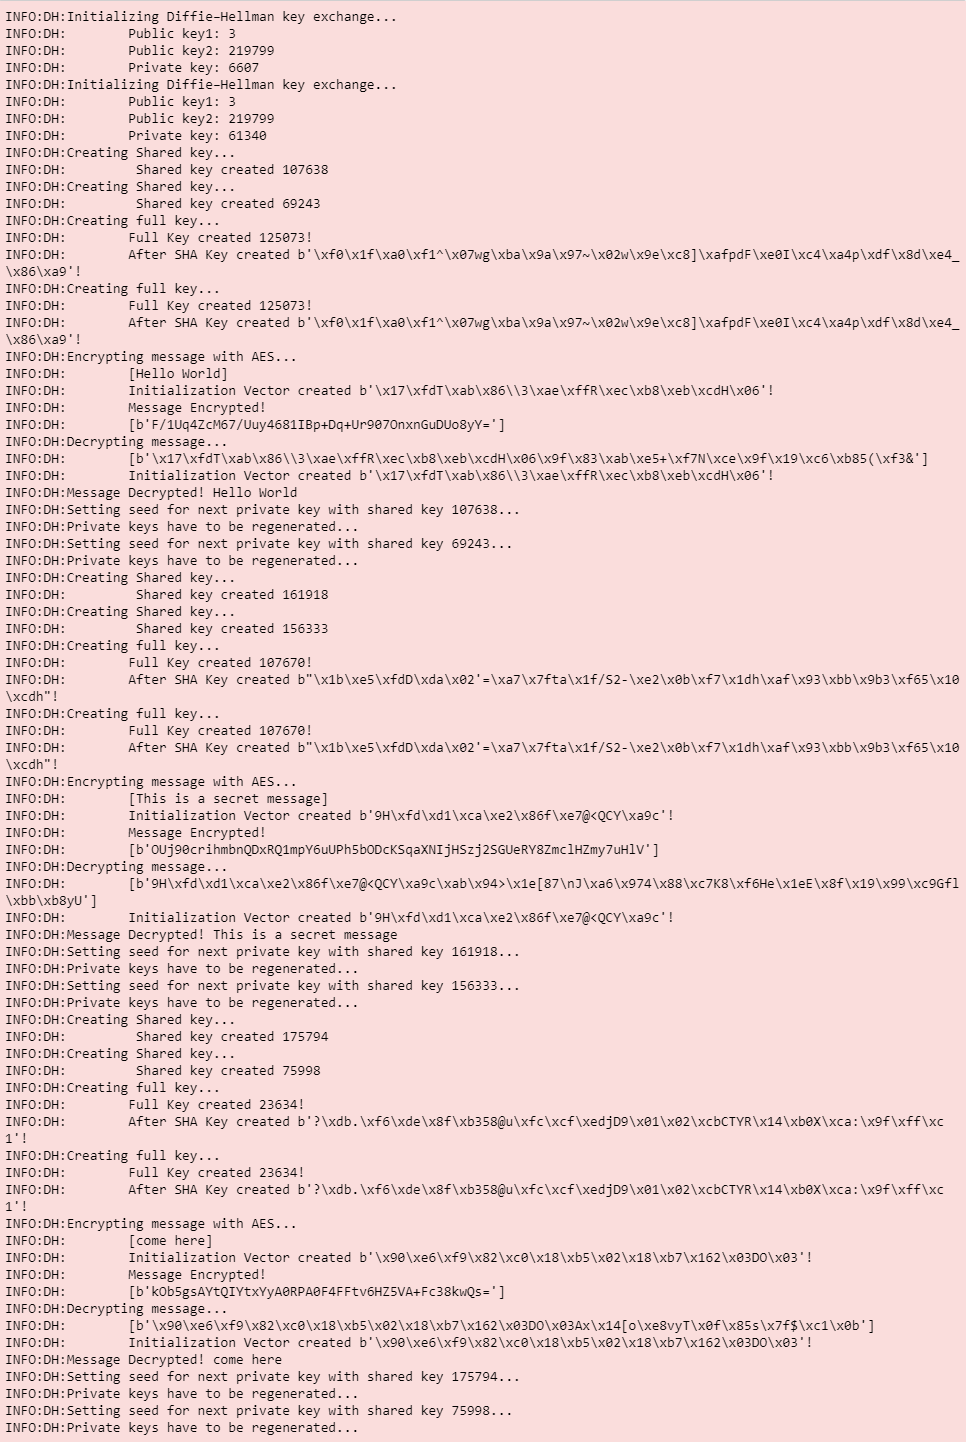
\includegraphics[width=0.8\textwidth]{assets/diffie_hellman_log.png}
    \caption{The log generated through running the emulated key exchange code.}
    \label{fig:DH_LOG}
\end{figure}
It is finally possible to confirm through this code emulation that the algorithms and key exchange are properly working. 16-bit prime key numbers were chosen to avoid slow runs on the code.

\subsubsection{Log files}
In the following images the log for each entity is presented.

\begin{figure}[H]
    \centering
    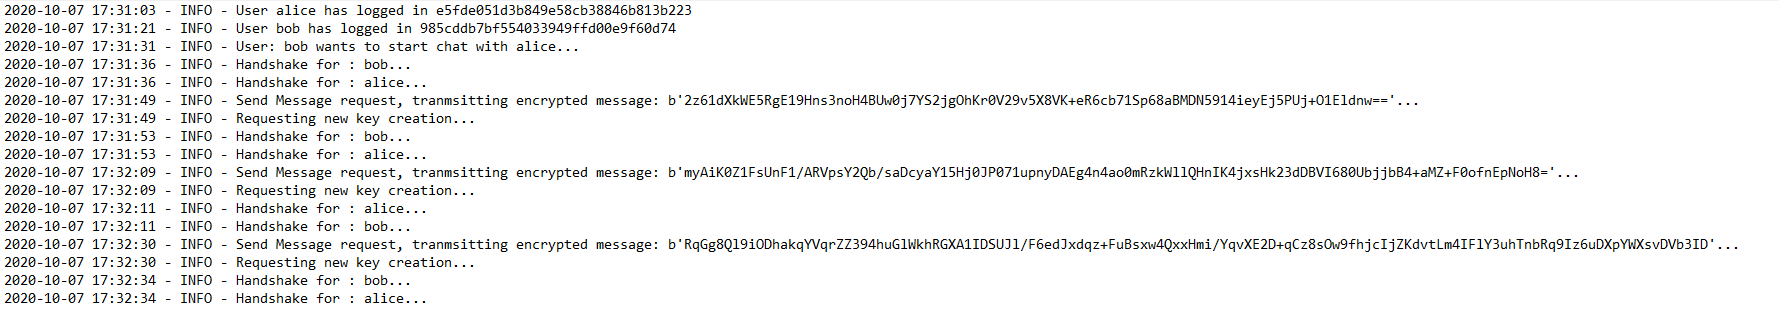
\includegraphics[width=0.9\textwidth]{assets/server_log.png}
    \caption{The log generated for the server entity.}
    \label{fig:SRV}
\end{figure}
\begin{figure}[H]
    \centering
    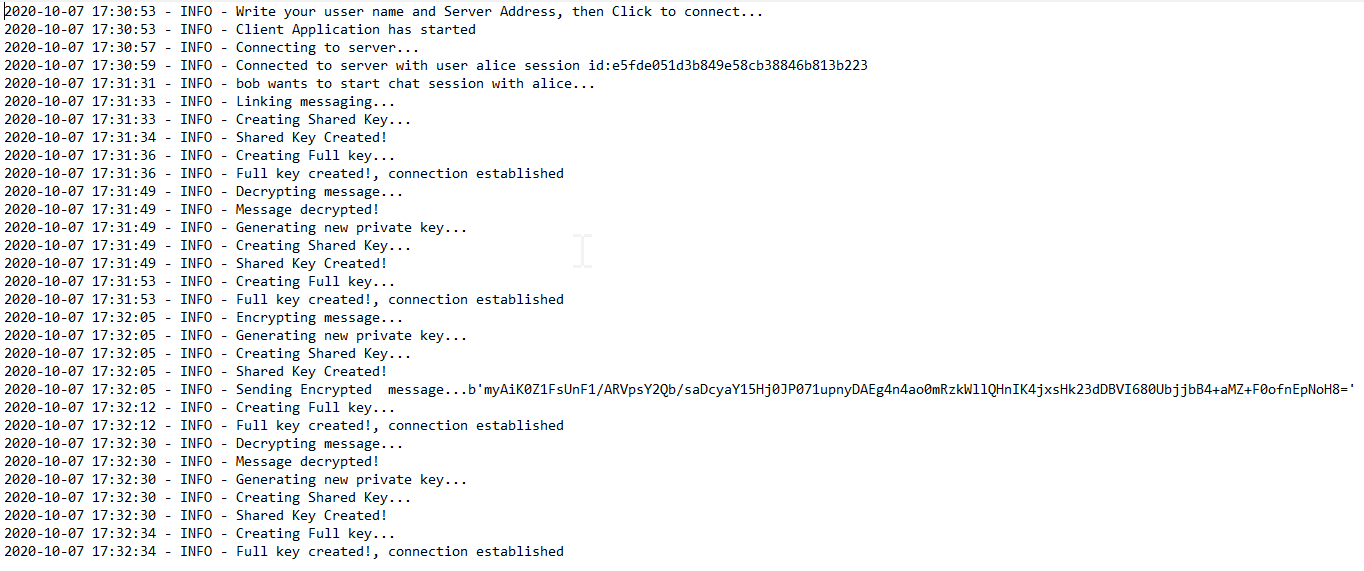
\includegraphics[width=0.9\textwidth]{assets/alice_log.png}
    \caption{The log generated for 'alice' client entity.}
    \label{fig:ALC}
\end{figure}
\begin{figure}[H]
    \centering
    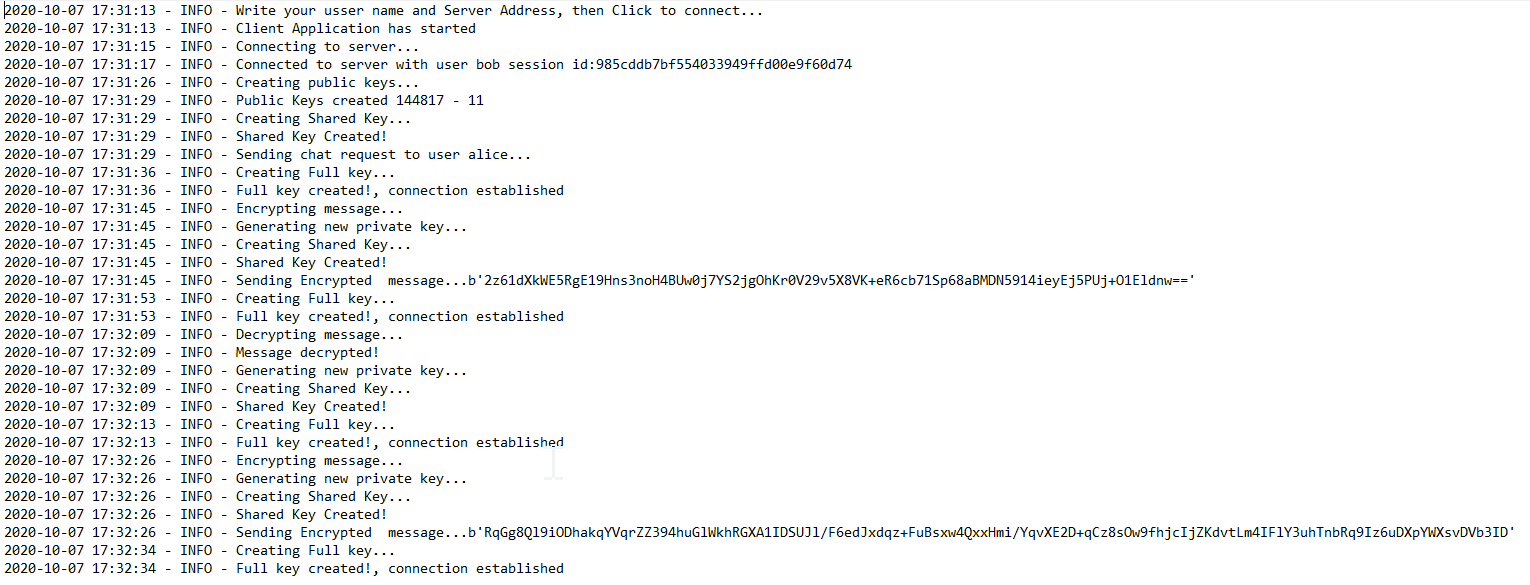
\includegraphics[width=0.9\textwidth]{assets/bob_log.png}
    \caption{The log generated for 'bob' client entity.}
    \label{fig:BOB}
\end{figure}


\section{Discussion}
\subsection{Part I}
The log files present in the Jupyter notebook allow to follow and see the different key exchange processes simulating two users sending messages each other. 
It is possible to confirm that all the algorithms work together by confirming that without sharing their private keys both end up having the same full key and later on manage to encrypt and decipher the information arriving to the same result.
\subsection{Part II}
It is possible to see that under no circumstance the messages are read by the server in raw text mode, it is agnostic of the key exchange mechanism and only acts as a communication coordinator.
Each client has its own implementation to generate their private keys and they do not share it, they just send the shared keys. The server is completely agnostic and works as a coordinator for both instances. Under the server log it is possible to visualize that it transmits the message encrypted.
The log files for the client show how they generate their own private keys based on pseudo random generation and later on send their shared key. Once any message is sent a new private key is generated.
\section{Conclusion}
During the realization of this assignment it was possible to emulate and build a simple encyption comunication application by building from scratch the algorithms for: Key Exchange (Diffie-Hellman), CSPRNG (BBS) and the use of other AES symmetric encryption algorithm to encrypt the messages.
Later on and through the use of Python language as well as socketio communication protocol it was possible to learn and confirm the importance of such encryption system for reliable and accurate communication as well as the considerable latency that strong encryption systems can generate. 
These tests were made on a normal computer without end-to-end communication, however the latency is perceptible for each communication mechanism. 

A very important lesson learned from this analysis is the realization that encryption algorithms are complex and they add an extra layer of complexity for building applications. That said, it is very important to have a quality control rule for communication processes and to think how far it is possible to get into these encryption systems without affecting the latency of the communication applications.

A video presentation has been elaborated and can be visualized \href{https://youtu.be/cKevoex-4h8}{in this link.}

\bibliographystyle{plainnat}
\bibliography{references}



\end{document}
